
\section{Monte Carlo Simulation}
\label{sec:cmsexperiment:simulation}



The Monte Carlo simulated events are produced via a chain of processes, which can be divided into three main stages, the event generation (GEN), the detector simulation (SIM), and the digitization (DIGI). 


\begin{figure}[ht]
    \centering
    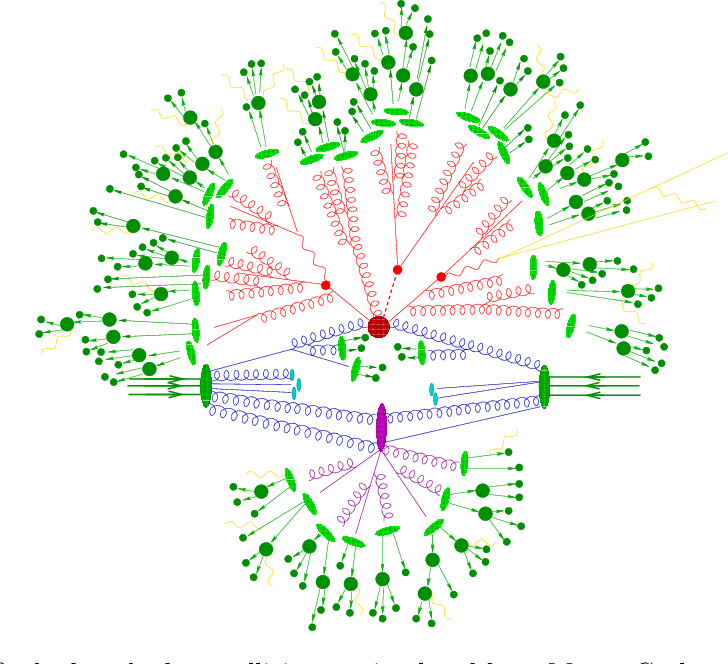
\includegraphics[trim={0 0.1cm 0 0}, clip, width=0.6\textwidth]{chapters/CMSExperiment/sectionMCSimulation/figures/ps.png}
    \caption{Physics processes happening in a proton-proton collision. The lower purple blob represents underline events. The upper purple blob shows the hard process with ISR before it and with FSR-PS-hadronization-decay after it. All of these processes are handled properly in the GEN stage by the generator and Pythia8. }
    \label{fig:cmsexperiment:simulation:collision}
\end{figure}

% GEN
GEN stage generates the lists of final state particles for the proton-proton collision events. The software can be summarized as ``generator+Pythia8". The event generation starts with initiating the generator with a configuration of the key input information, such as the beam parameters, the parton distribution functions, and the QFT models for the signal. Common generator software includes Madgraph, Powheg, HERWIG, SHERPA, Pythia8. Upon initiation, based on the provided QFT model, the generator calculates the matrix element and cross-section of the signal hard process perturbatively at either leading order or next leading order with respective to the coupling constant. Then it generates the signal hard process according to the calculated differential cross-section. Possible ISR and FSR gluons and photons are also included. Next, for all outcoming particles from the generator, Pythia8 is used to perform the parton shower, hadronization, and decay of unstable particles. In addition, Pythia8 also adds underline events (UE) to the signal hard process according to certain UE tuning. The underline events are QCD scatterings at the same proton-proton vertex as the hard process. Figure~\ref{fig:cmsexperiment:simulation:collision} illustrates the physics processes happening during a proton-proton collision, all of which are properly treated in the GEN stage with ``generator+Pythia8".




% sim-Pileup-DIGA
The SIM stage uses GEANT4 to simulate the energy deposits, known as hits, of the final state particles in the CMS detector. A detailed model of the CMS detector, including magnetic field, electronics, cables, and supporting mechanics, is created in the GEANT4.  Pile-up events, also referred to as MinBias (MB) events, are separately produced with the same GEN-SIM pipeline beforehand. According to the instant luminosity and expected average number of PUs, the MB events are mixed with the signal events after the GEN-SIM stage. The DIGI stage simulates the response to hits of the detector readout electronics. The purpose is to produce the most realistic simulation of the collected data as close as possible to the real CMS detector. After the DIGI stage, the exactly same reconstruction and post-processing software are used for MC events as the data events. 